\section{Anhang}

\renewcommand{\arraystretch}{1.5}
\subsection{Laplace-Transformation}
    \begin{minipage}[t]{0.48\textwidth}
        \textbf{Korrespondenzen der Laplace-Transformation}\\
        \begin{tabularx}{\textwidth}{|X|X|}
            \hline
            \textbf{x(t)} & \textbf{X(s)} \\
            \hline
            \(\delta(t)\), Dirac & 1 \\
            \hline
            \(1\), \(\sigma(t)\), Sprung & \(\frac{1}{s}\) \\
            \hline
            \(t^n\) & \(\frac{n!}{s^{n+1}}\) \\
            \hline
            \(\sin \omega t\) & \(\frac{\omega}{s^2 + \omega^2}\) \\
            \hline
            \(\cos \omega t\) & \(\frac{s}{s^2 + \omega^2}\) \\
            \hline
            \(e^{-at}\) & \(\frac{1}{s+a}\) \\
            \hline
            \(1-e^{-at}\) & \(\frac{a}{s(s+a)}\) \\
            \hline
            \(t^n \cdot e^{-at}\) & \(\frac{n!}{(s+a)^{n+1}}\) \\
            \hline
            \(e^{-at} \cdot \sin \omega t\) & \(\frac{\omega}{(s+a)^2 + \omega^2}\) \\
            \hline
            \(e^{-at} \cdot \cos \omega t\) & \(\frac{s+a}{(s+a)^2 + \omega^2}\) \\
            \hline
        \end{tabularx}
    \end{minipage}%
    \hfill
    \begin{minipage}[t]{0.48\textwidth}
        \textbf{Rechenregeln der Laplace-Transformation}\\
        \begin{tabularx}{\textwidth}{|X|X|}
            \hline
            \textbf{x(t)} & \textbf{X(s)} \\
            \hline
            \(\alpha x_1(t) + \beta x_2(t)\) & \(\alpha X_1(s) + \beta X_2(s)\) \\
            \hline
            \(\frac{d}{dt}x(t)\) & \(sX(s) - x(0)\) \\
            \hline
            \(\int_{0}^{t} x(\tau) d\tau\) & \(\frac{X(s)}{s}\) \\
            \hline
            \(x(t-T_t) \sigma(t-T_t)\) & \(e^{-sT_t} X(s)\) \\
            \hline
            \(e^{-at} x(t)\) & \(X(s+a)\) \\
            \hline
            \(t \cdot x(t)\) & \(-\frac{d}{ds} X(s)\) \\
            \hline
            \(x(t) * x_2(t)\) & \(X_1(s) \cdot X_2(s)\) \\
            \hline
        \end{tabularx}
        \vspace{12pt}
        \begin{tabularx}{\textwidth}{|X|}
            \hline
            Grenzwertsätze: \\
            \hline
            Anfangswertsatz: \(\lim_{t \to 0} x(t) = \lim_{s \to \infty} sX(s)\) \\
            Endwertsatz: \(\lim_{t \to \infty} x(t) = \lim_{s \to 0} sX(s)\) (max. 1 Pol im Ursprung, Rest in der linken Halbebene)\\
            \hline
        \end{tabularx}
    \end{minipage}

\subsection{Elementare Systeme}
    \centering
    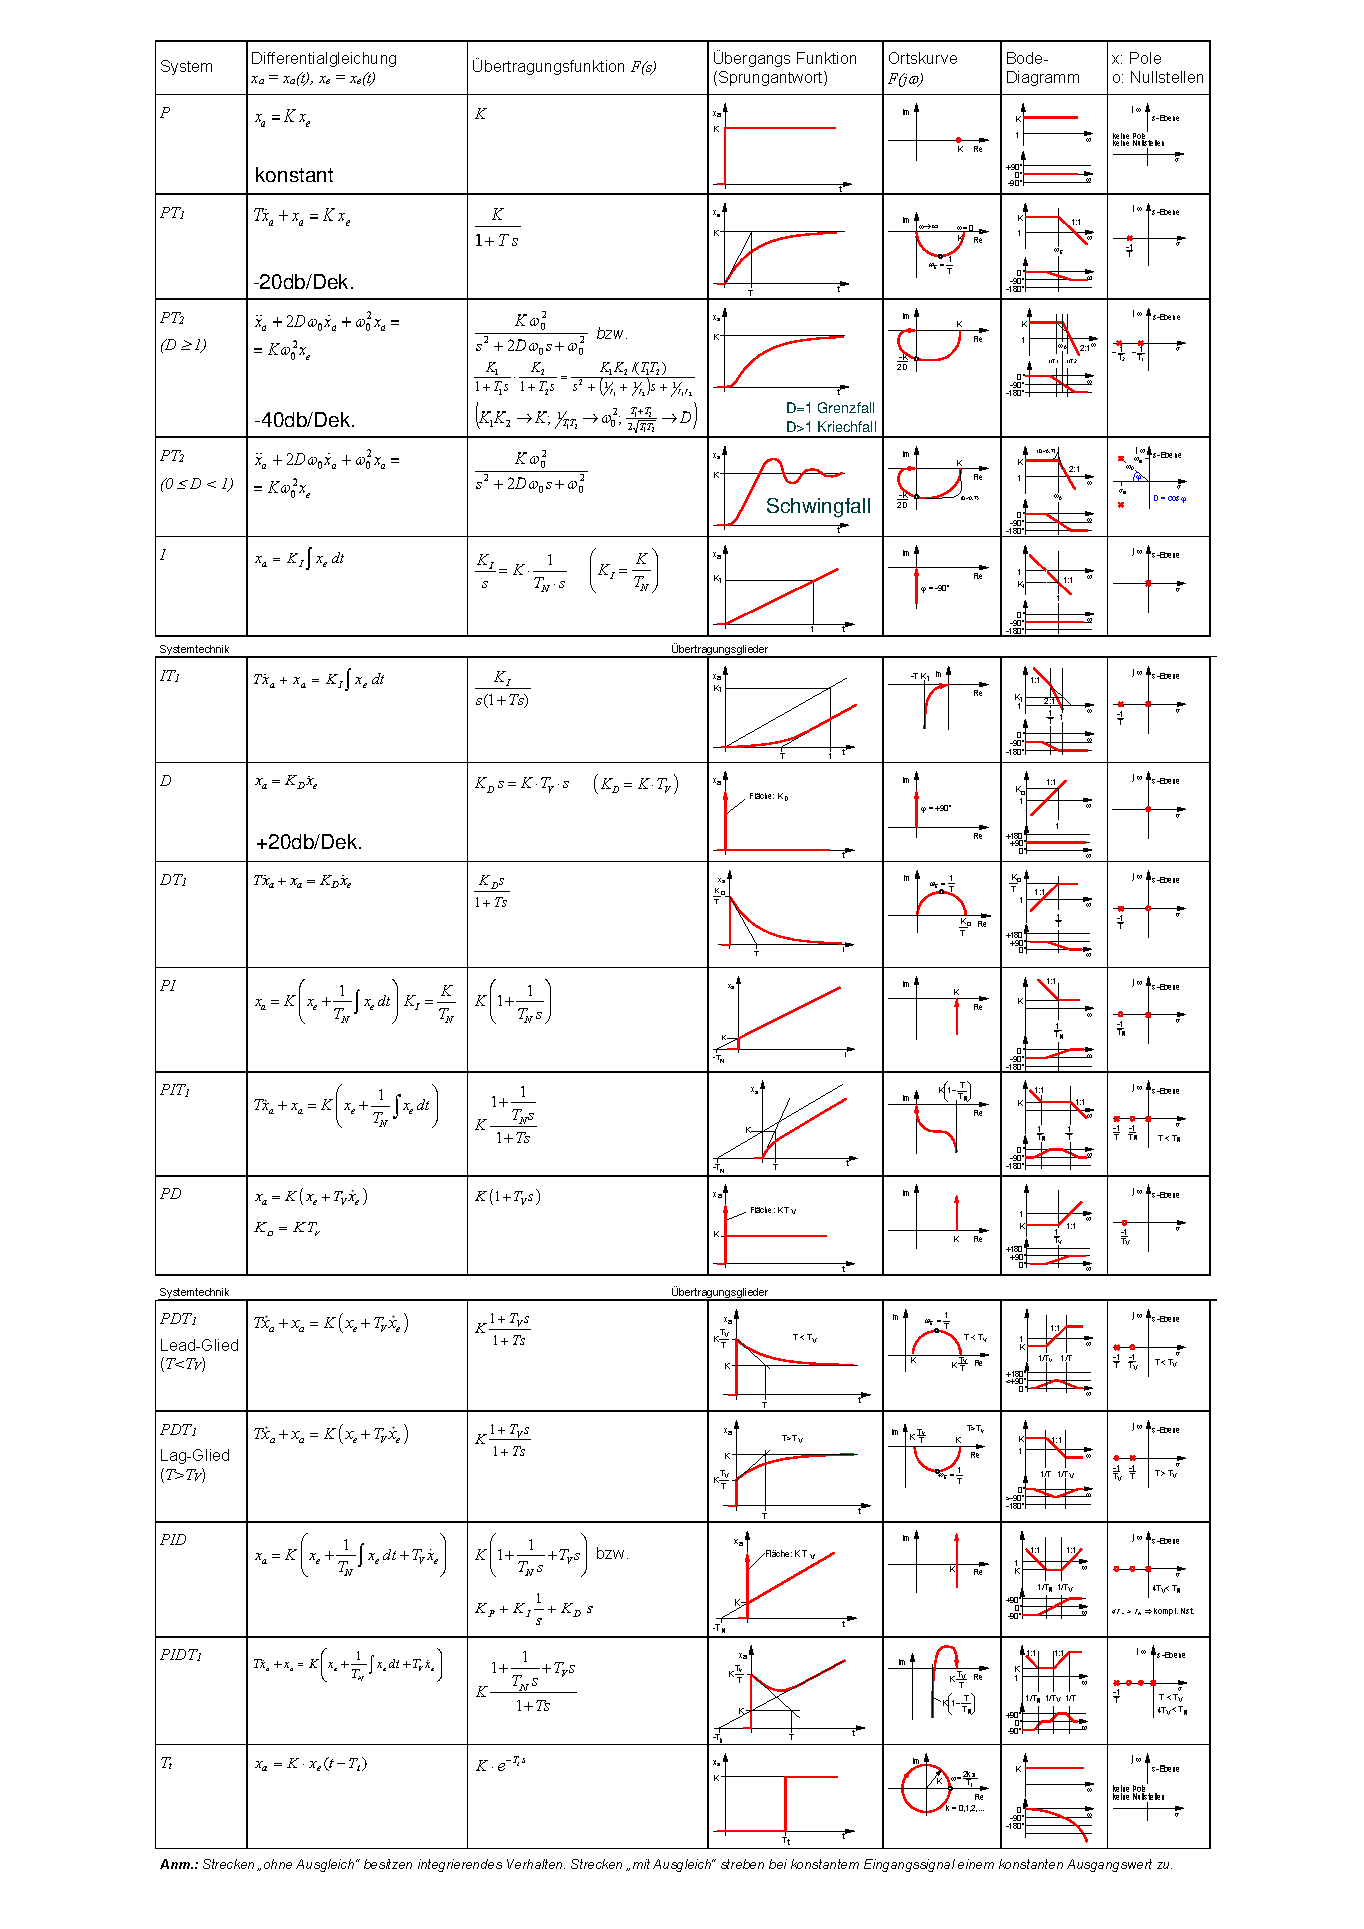
\includegraphics[width=0.8\textwidth]{Figures/Systeme.pdf}
